\appendix

\section{Element Types within LISA}
Here are shown the the visual specifications LISA provides for the ordering and layout of nodes for defining each type of element supported. Each of these types can be classified using the 

\begin{figure}[ht]
\centering
\begin{subfigure}{.5\textwidth}
  \centering
  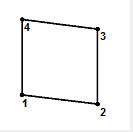
\includegraphics[width=0.3\linewidth]{../Graphics/LISA-quad4.png}
  \caption{quad4 element}
  \label{fig:sub1}
\end{subfigure}%
\begin{subfigure}{.5\textwidth}
  \centering
  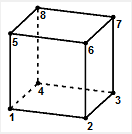
\includegraphics[width=0.3\linewidth]{../Graphics/LISA-hex8.png}
  \caption{hex8 element}
  \label{fig:sub2}
\end{subfigure}
\label{fig:test}
\end{figure}


\begin{figure}[ht]
\centering
\begin{subfigure}{.5\textwidth}
  \centering
  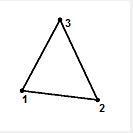
\includegraphics[width=0.3\linewidth]{../Graphics/LISA-tri3.png}
  \caption{Specification for node ordering of tri3 element within LISA}
  \label{fig:sub1}
\end{subfigure}%
\begin{subfigure}{.5\textwidth}
  \centering
  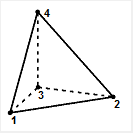
\includegraphics[width=0.3\linewidth]{../Graphics/LISA-tet4.png}
  \caption{tet4 element}
  \label{fig:sub2}
\end{subfigure}
\label{fig:test}
\end{figure}


\begin{figure}[ht]
\centering
\begin{subfigure}{.5\textwidth}
  \centering
  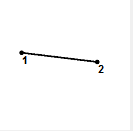
\includegraphics[width=0.3\linewidth]{../Graphics/LISA-line2.png}
  \caption{line2 element}
  \label{fig:sub1}
\end{subfigure}%
\begin{subfigure}{.5\textwidth}
  \centering
  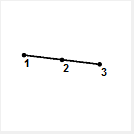
\includegraphics[width=0.3\linewidth]{../Graphics/LISA-line3.png}
  \caption{line3 element}
  \label{fig:sub2}
\end{subfigure}
\label{fig:test}
\end{figure} 

%\section{Calculating Centripetal Force For Paper Mill}
%Assuming a constant speed of the paper mill disk at  the following standard calculation was done to compute a forces that could be specified for different elements in order to simulate the effects on the model.

%F = m $\omega^2$ r\\ 

%where: \\ 
%m - mass of object \\ 
%r - radius from centre \\ 
%$\omega$ - angular velocity (radians per second)

%Using the following values for each variable for the plates forming the outside of the paper mill disk the force could be calculated as:

%mass- paper mill is made of steel with each plate having a volume of approximately $24cm^3$ which gives a mass of
%188 grams


\section{Unit Testing}
%Unit tests to validate the correctness of key functionality



\cite{Centripetal}

\section{Input and output files}
Below can be seen the format of the input files for the system, a LISA .liml and a .json edge definition file\\

\begin{figure}[h!!]
\centering
\begin{subfigure}{.5\textwidth}
  \centering
  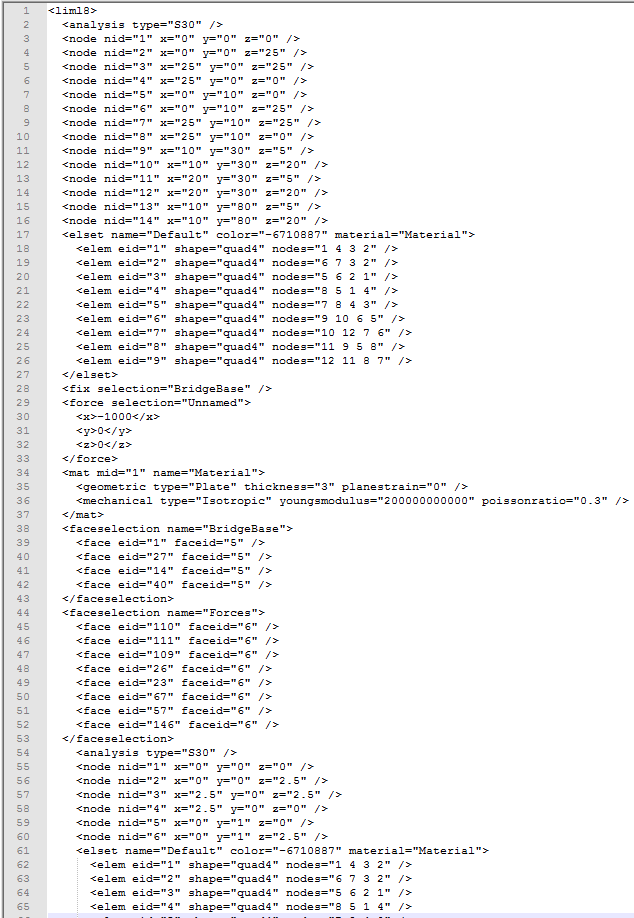
\includegraphics[width=0.6\linewidth]{../Graphics/limlFileLayout.png}
  \caption{Cut down .liml file to show general content which largely defined the schema for the systems data model}
  \label{fig:sub1}
\end{subfigure}%
\begin{subfigure}{.5\textwidth}
  \centering
  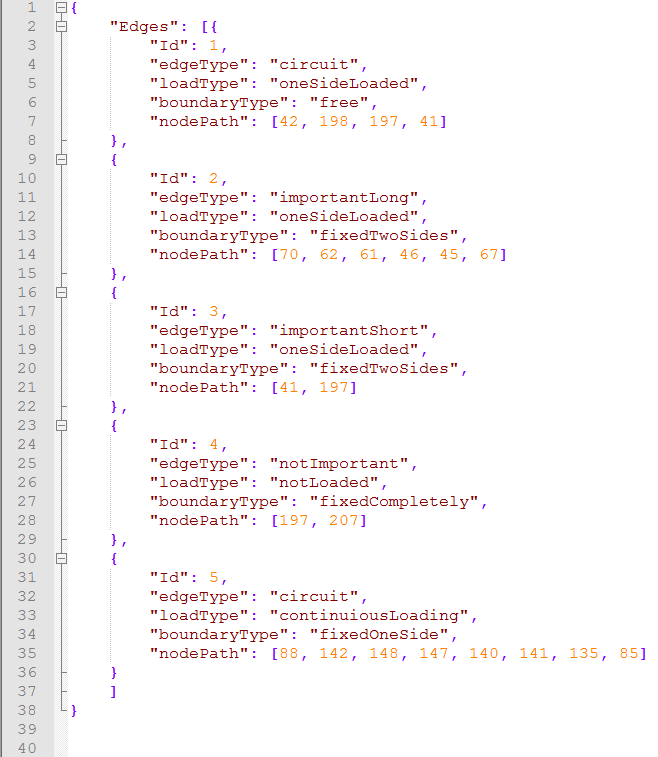
\includegraphics[width=0.8\linewidth]{../Graphics/jsonEdgeFileLayout.png}
  \caption{A json file containing the edges of interest specified by an engineer, this is parsed and the rules are applied to determine the models meshing based on the input}
  \label{fig:sub2}
\end{subfigure}
\label{fig:test}
\end{figure}


\section{Project Layout in Solution Explorer}
Below show the Visual Studio Solution Explorer which provides a general idea of the layout of the project with namespace hierarchies from within an IDE.

\begin{figure}[h!!]
  \centerline{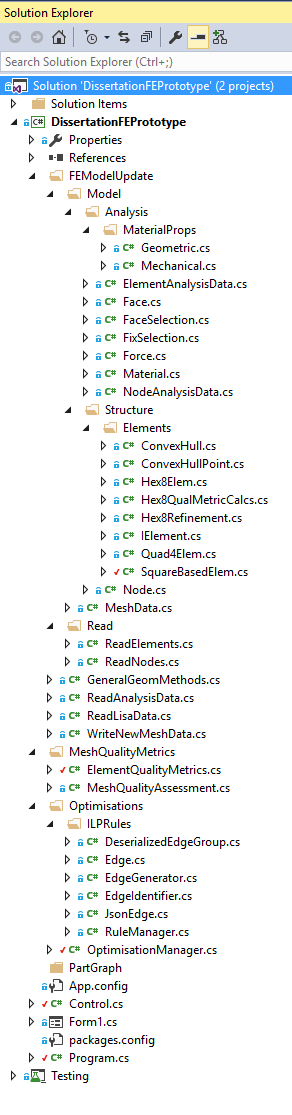
\includegraphics[width=60mm, scale=0.5]{../Graphics/VSolutionExplorer.png}}
  \caption{The metrics calculated by visual studio for all high level modules in the system}
\end{figure}


\section{Software Quality Metrics}
\begin{figure}[h!!]
  \centerline{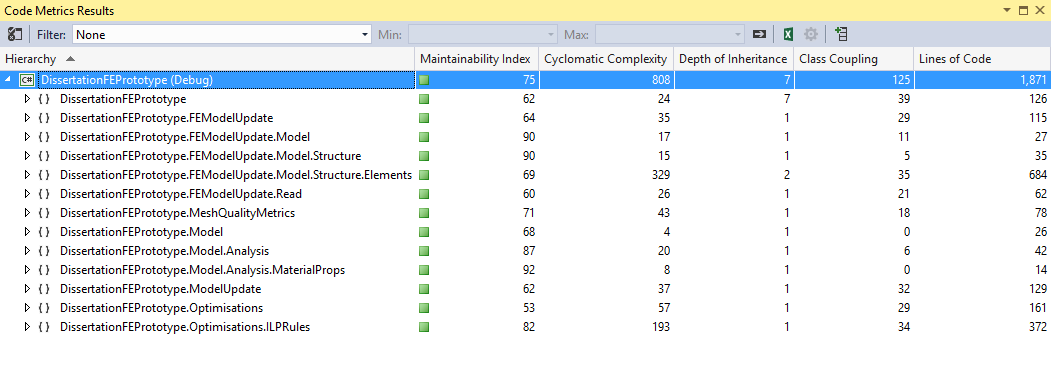
\includegraphics[width=165mm, scale=0.5]{../Graphics/softwareQualityMetrics.png}}
  \caption{The metrics calculated by visual studio for all high level modules in the system}
\end{figure}

\begin{figure}[h!!]
  \centerline{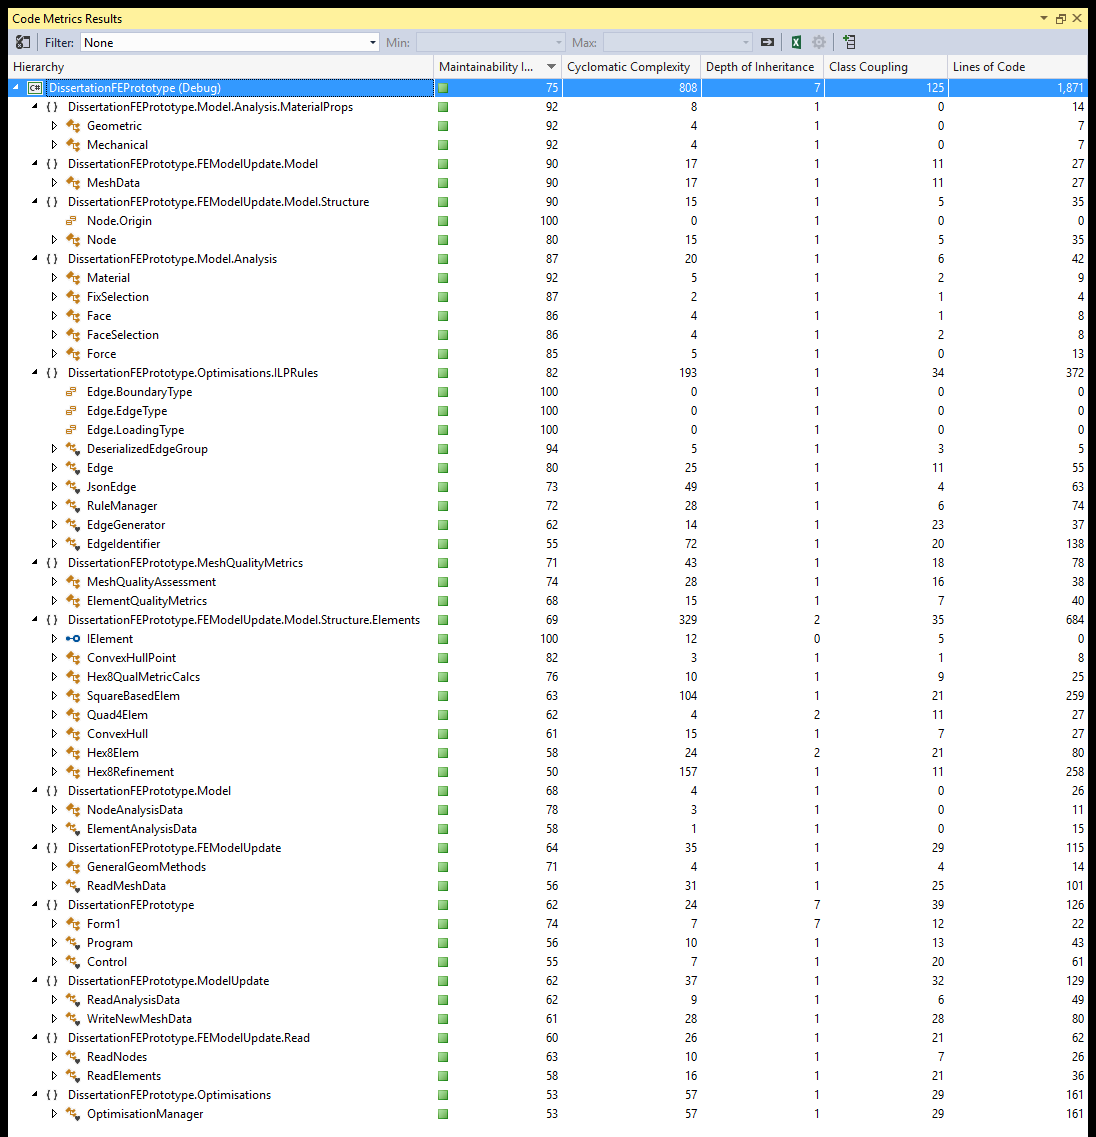
\includegraphics[width=165mm, scale=0.5]{../Graphics/qualityMetricsExpanded.png}}
  \caption{The metrics calculated by visual studio for the all classes in the final system}
\end{figure}
%


\section{Bridge Cross Loading Simulation Results}
Below can be seen the results of executing both the heuristics and the stress refinement method on the suspension bridge model when loads are placed against the base of the bridge in the negative x direction.

\subsection{Heuristic Refinement}

\begin{figure}[h!!]
\centering
\begin{subfigure}{.5\textwidth}
  \centering
	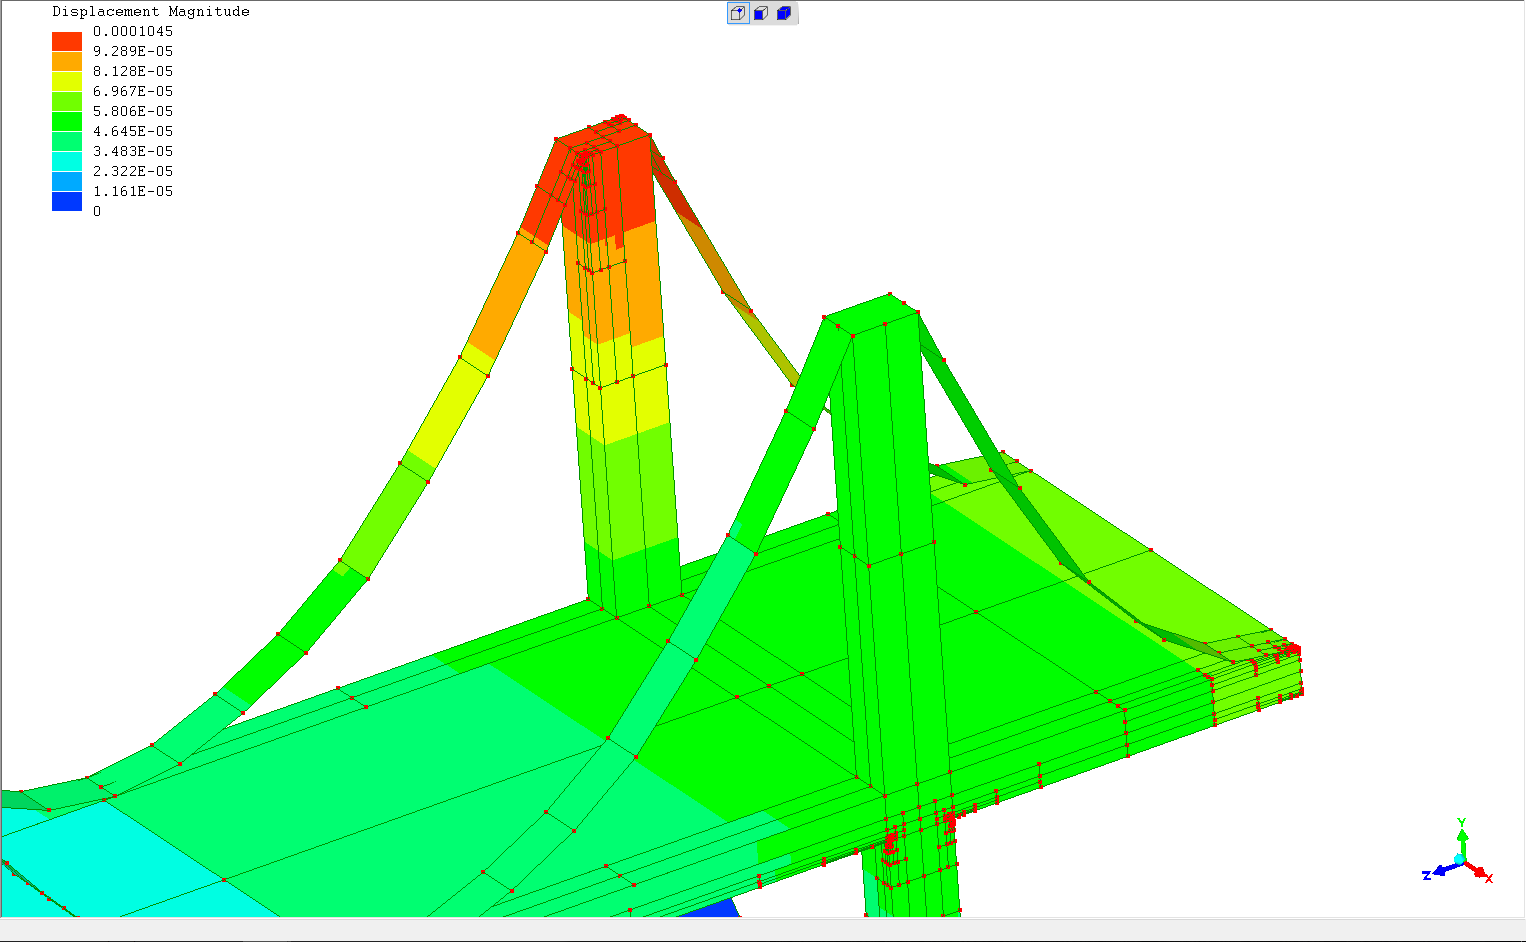
\includegraphics[width=80mm, scale=0.5]{../Graphics/BridgeCrossLoading/bestEdgeSpecResults.png}
  \caption{Important edges specified effectively to facilitate preemptive meshing of area which undergoes high displacement and thus stress}
  \label{fig:sub1}
\end{subfigure}%
\begin{subfigure}{.5\textwidth}
  \centering
  \centerline{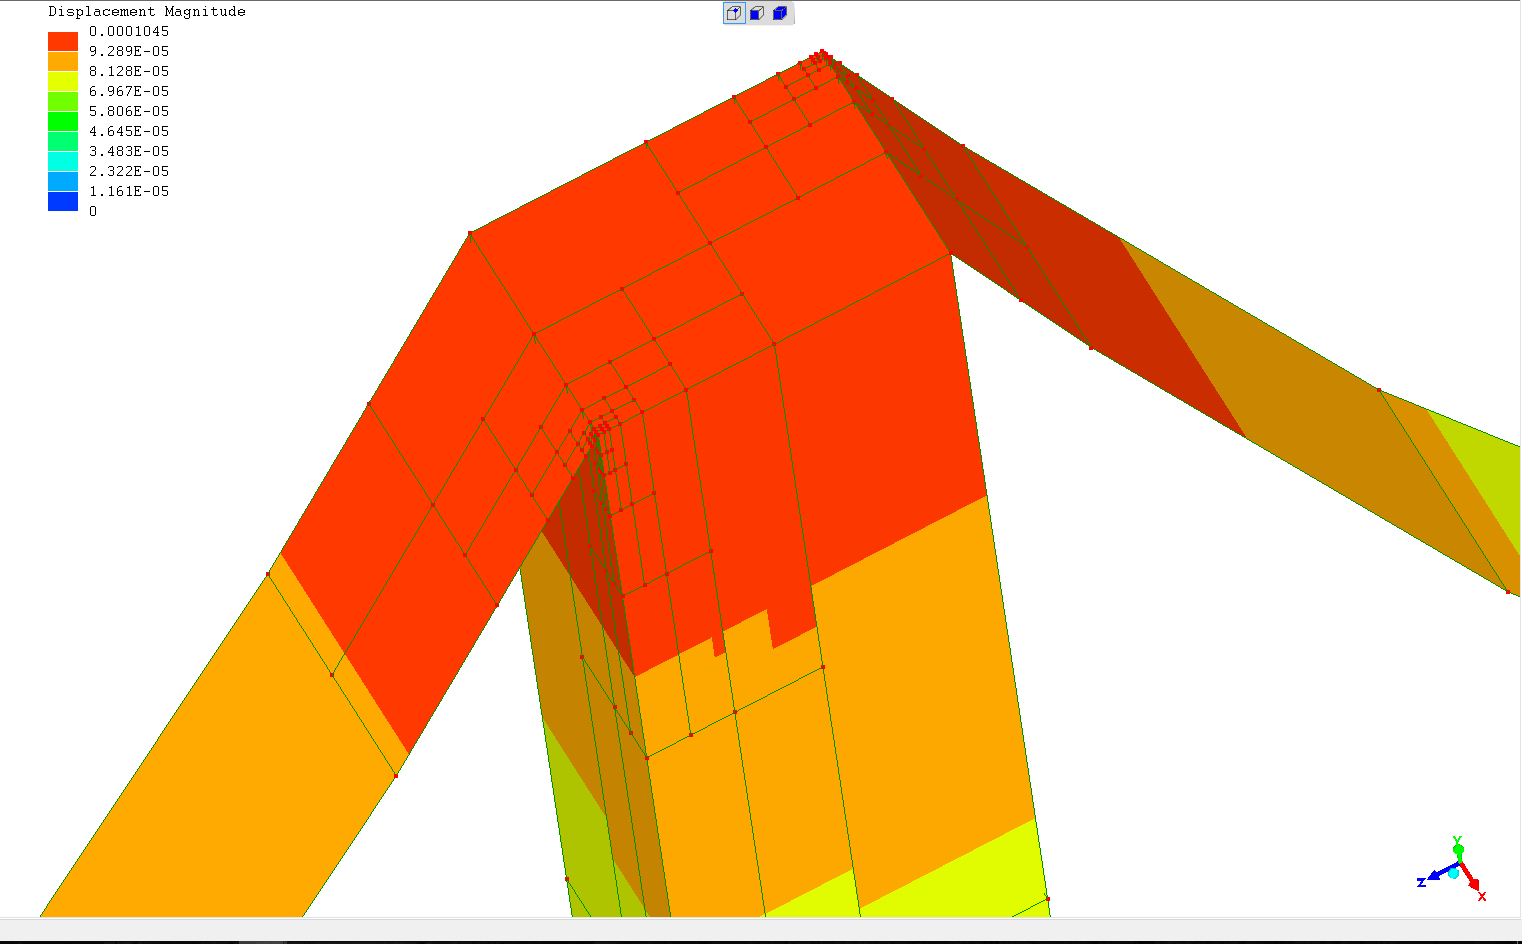
\includegraphics[width=80mm, scale=0.5]{../Graphics/BridgeCrossLoading/bestEdgeSpecResultsCloseUp.png}}
  \caption{Close up view of refinement for high displacement areas }
  \label{fig:sub2}
\end{subfigure}
\label{fig:test}
\end{figure}


\begin{figure}[h!!]
  \centerline{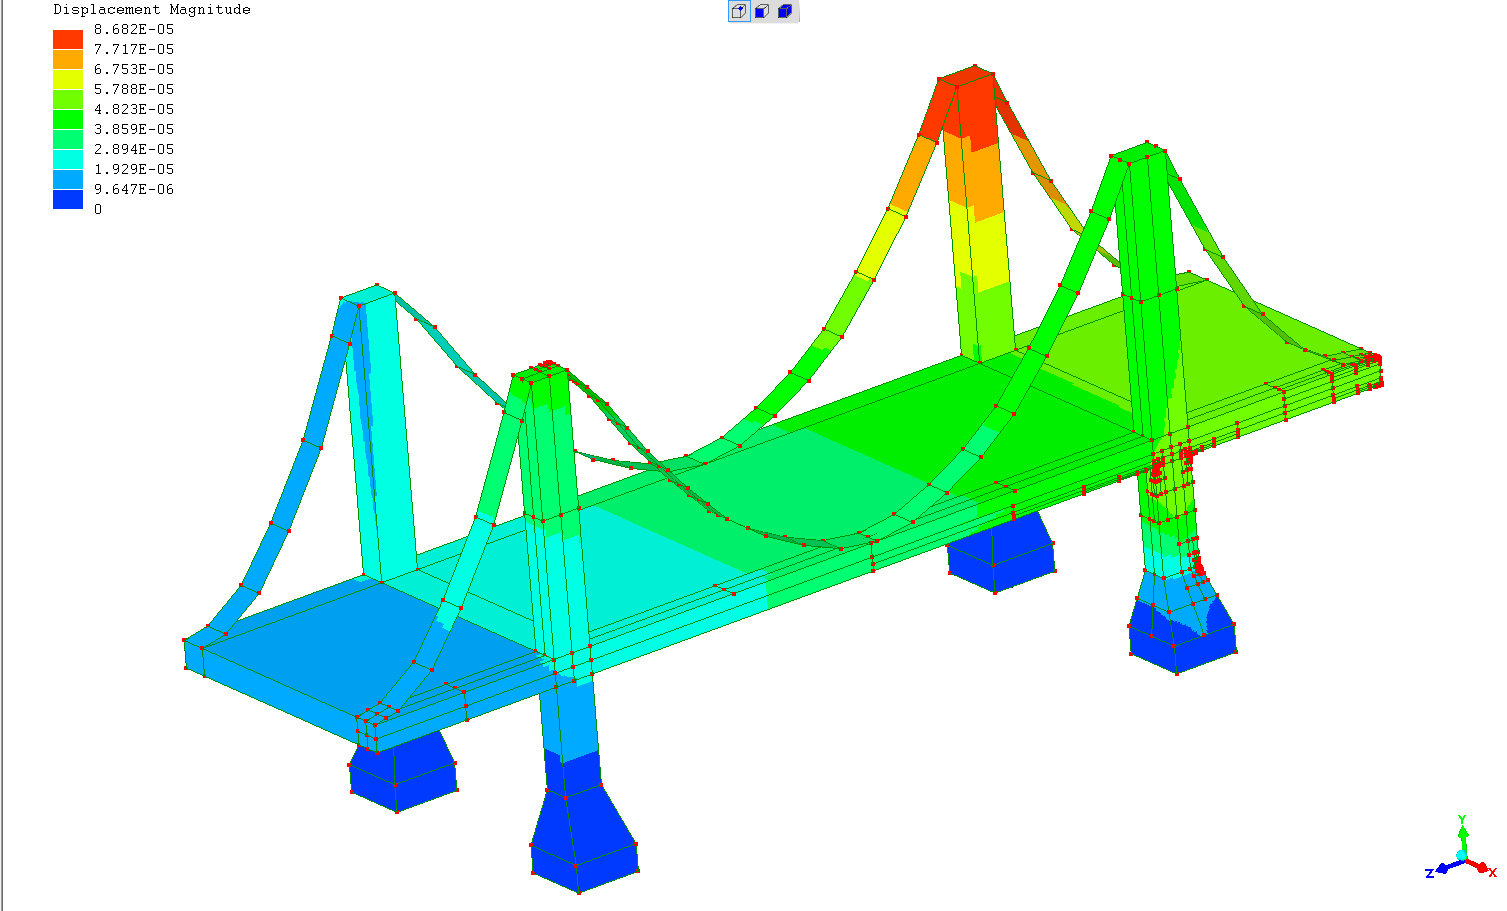
\includegraphics[width=165mm, scale=0.5]{../Graphics/BridgeCrossLoading/okEdgeSpecResults.png}}
  \caption{Important edges more poorly specified missing high displacement region on top of furthest suspension bridge tower}
\end{figure}

\section{Stress Refinement}
\begin{figure}[h!!]
  \centerline{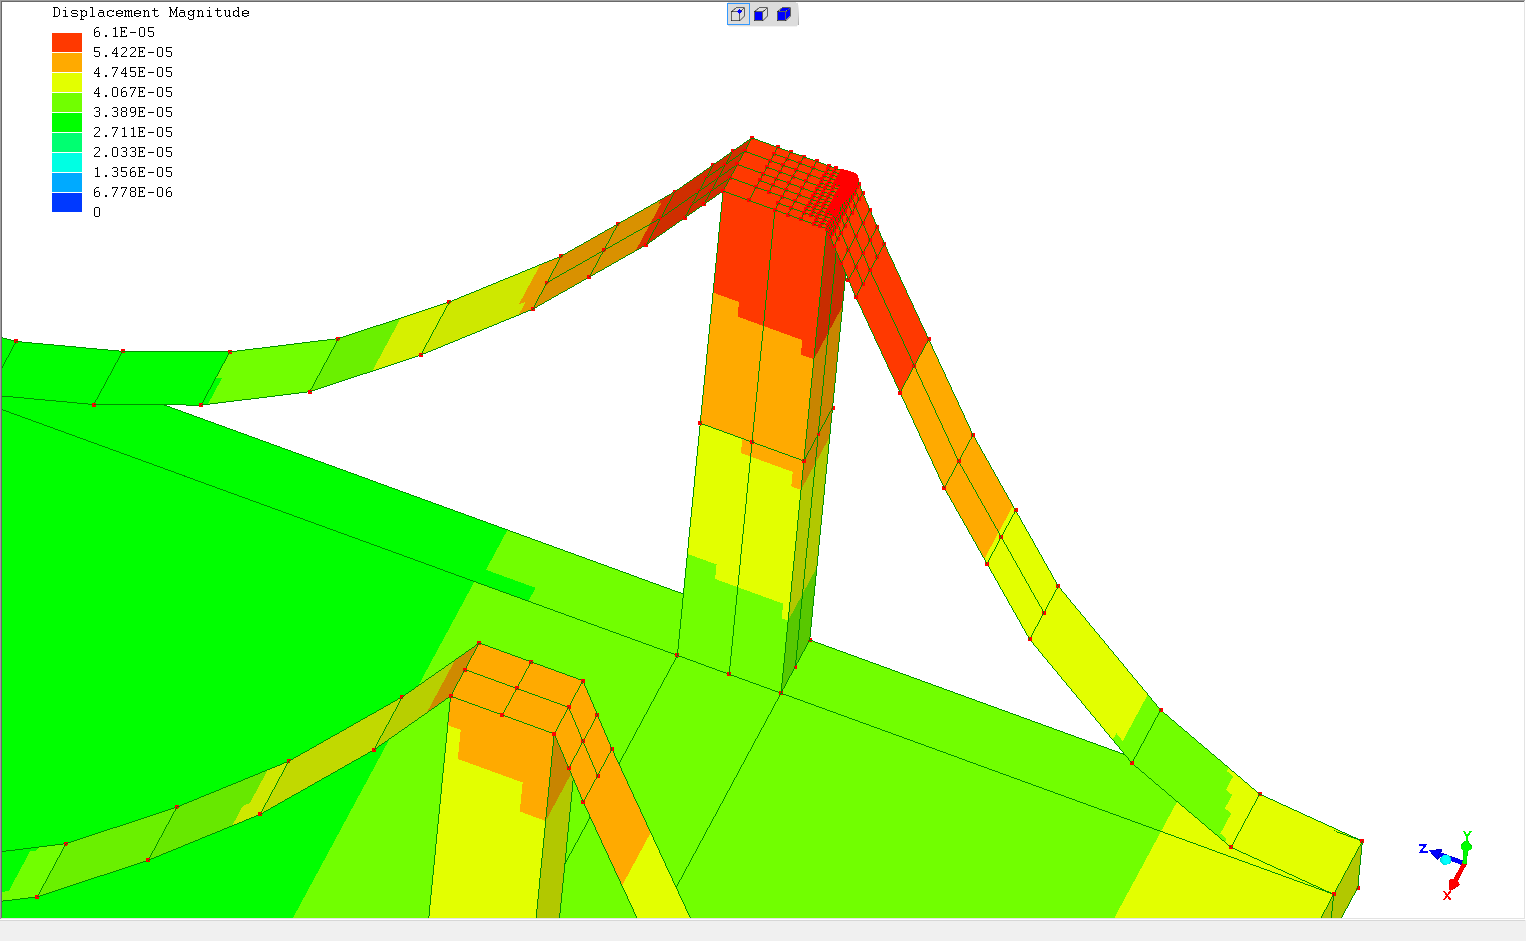
\includegraphics[width=165mm, scale=0.5]{../Graphics/BridgeCrossLoading/the90thPercentileRefinement.png}}
  \caption{Iterative stress/ displacement refinement method used to focus meshing on the top 6\% most displaced region of model}
\end{figure}

\begin{figure}[h!!]
  \centerline{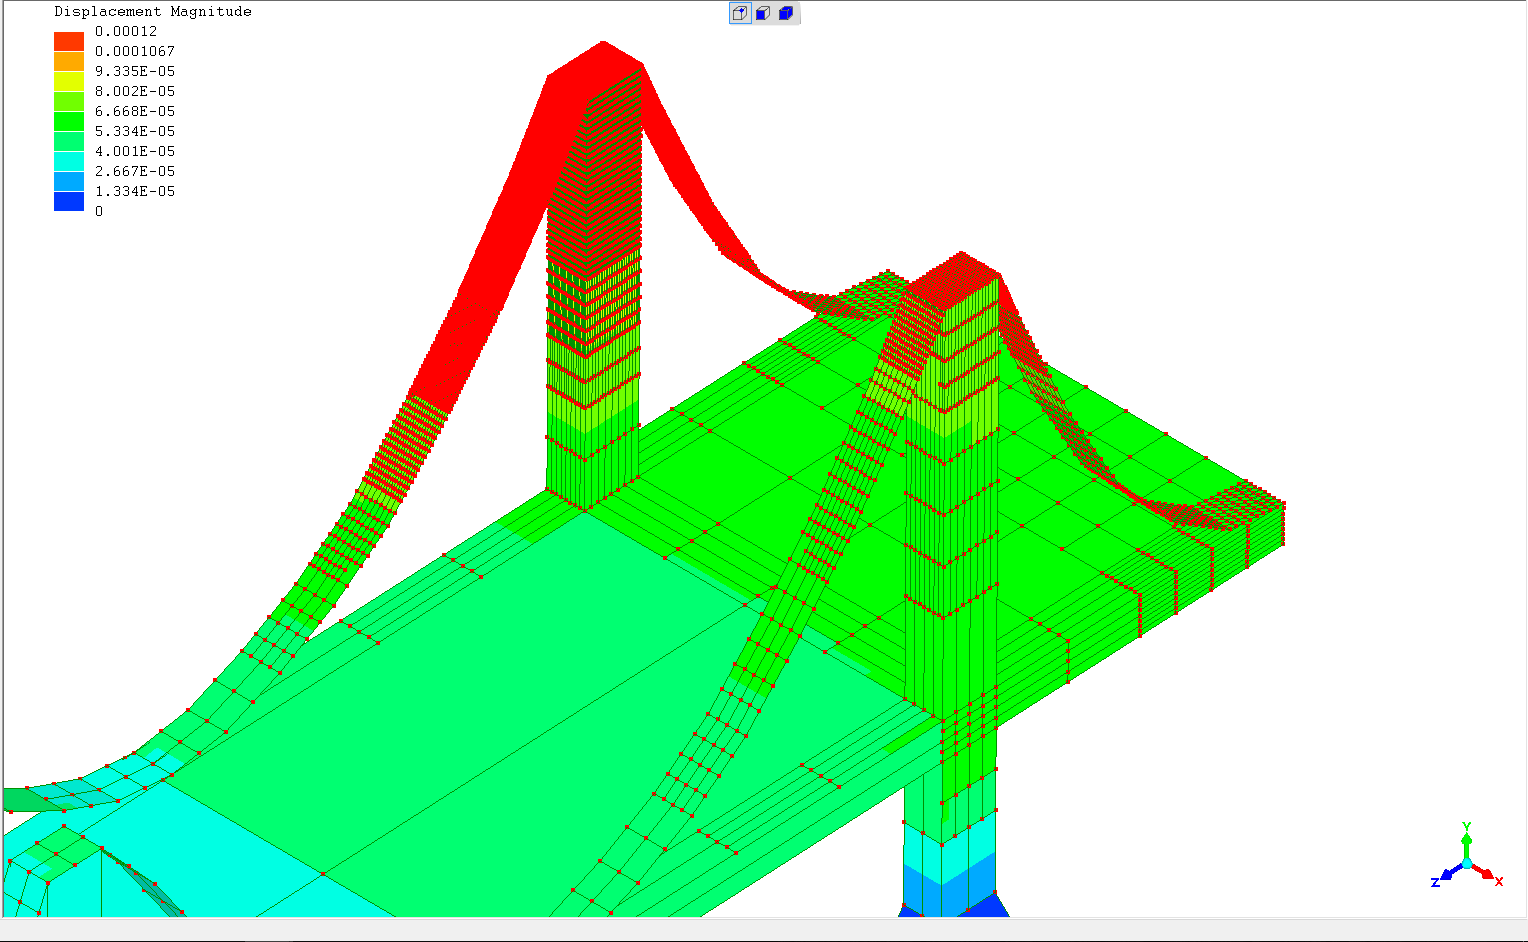
\includegraphics[width=165mm, scale=0.5]{../Graphics/BridgeCrossLoading/aboveAverageRefinement2.png}}
  \caption{Iterative refinement of high displacement but with the remesh threshold specified as the average displacement across the whole model. A consequence of this is the gradient of refinement fidelity that can be seen corresponding to the importance of that part of the structure}
\end{figure}


\begin{figure}[h!!]
  \centerline{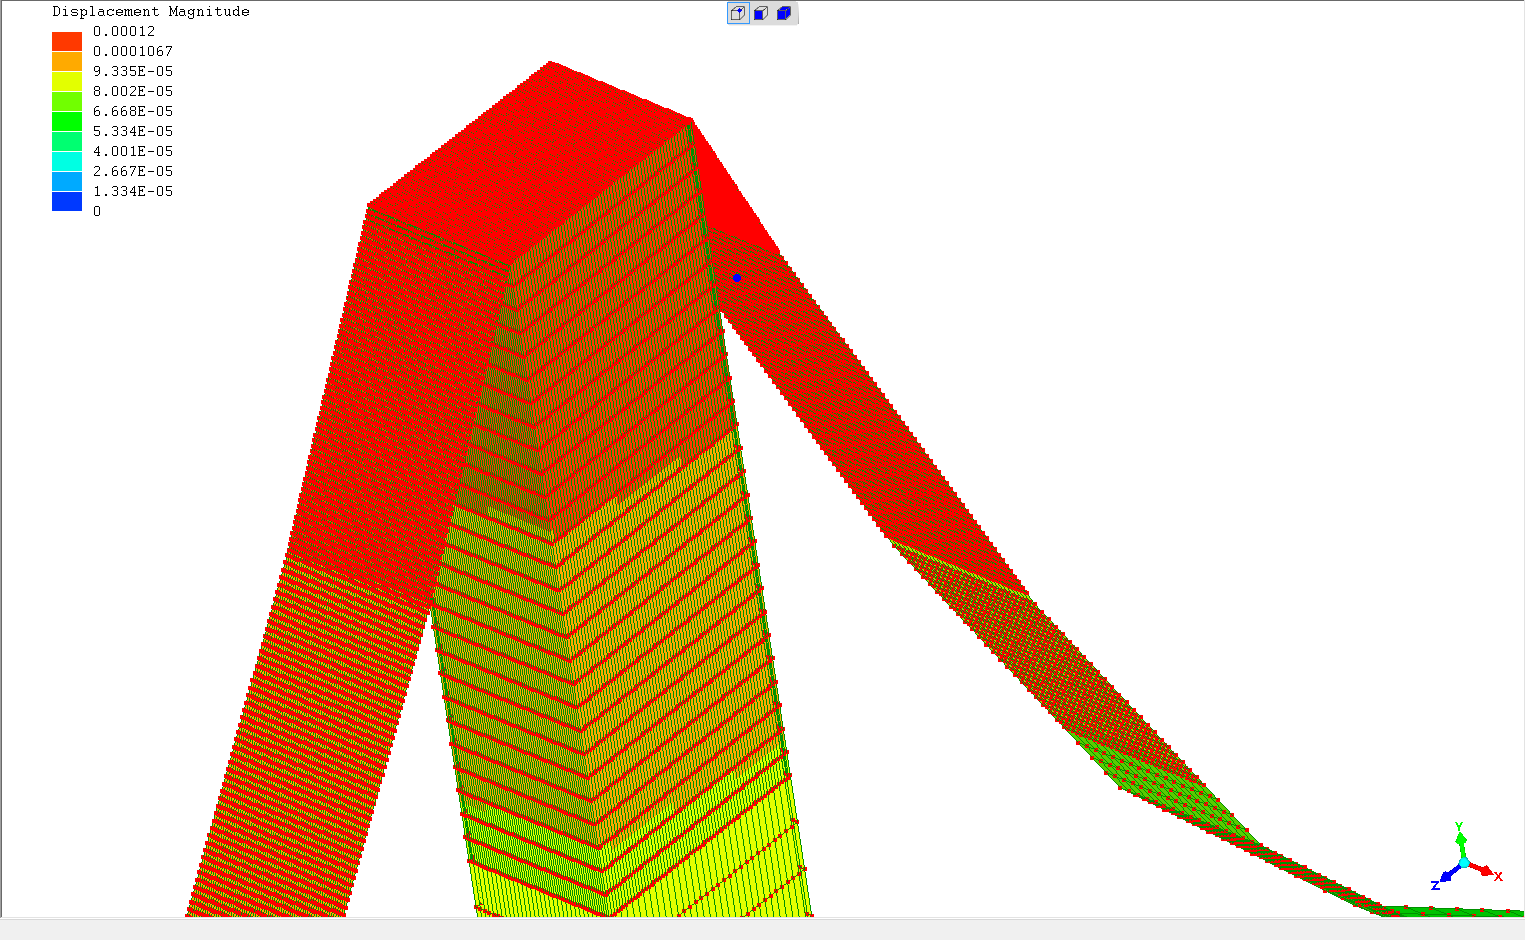
\includegraphics[width=165mm, scale=0.5]{../Graphics/BridgeCrossLoading/aboveAverageRefinement.png}}
  \caption{The metrics calculated by visual studio for the all classes in the final system}
\end{figure}
%\end{changemargin}


\section{Bridge Base Loading Simulation Results}

\section{Paper Mill Simulation Results}

\newpage  
\section{Gantt Chart for Project Time Management}
\pagestyle{empty}
\begin{landscape}
\vspace*{1cm}
\hspace*{-3cm}
\begin{figure}
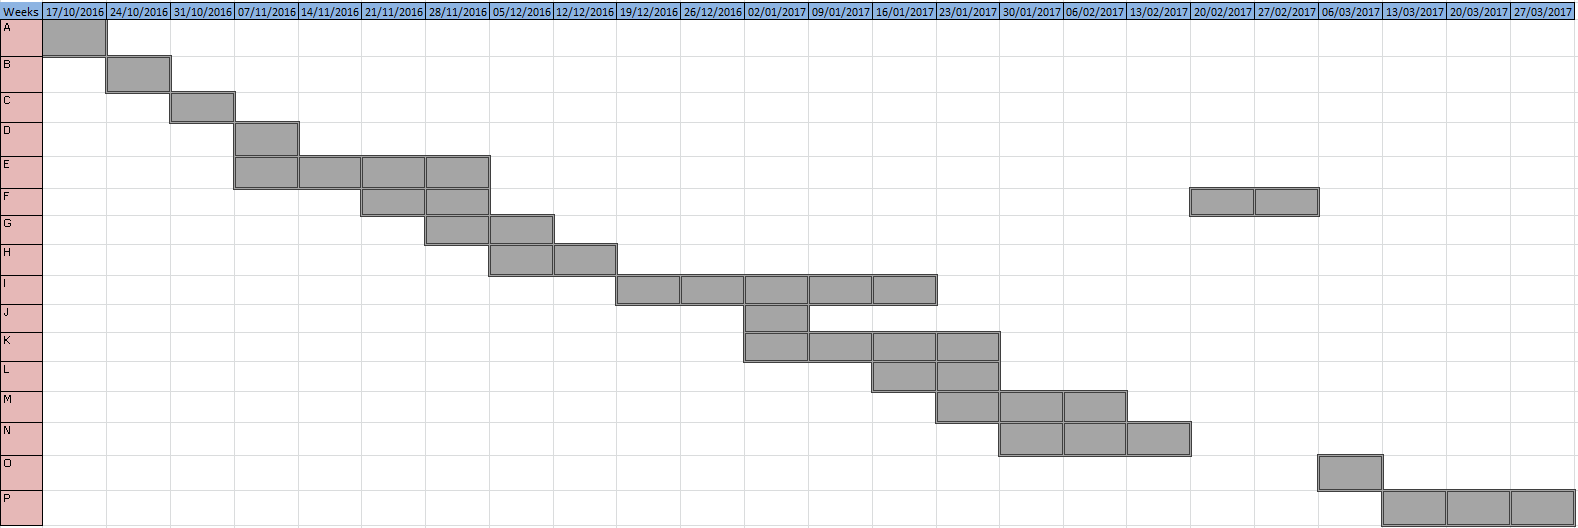
\includegraphics[width =700px, height=300px]{../Graphics/TimePlanUpdated2.png} \par
\end{figure}
\hspace*{-1cm}
\end{landscape}

